\lhead{\textbf{Basic Algorithms, Fall 2024 \\ CSCI-UA.0310-001}}
\chead{\Large{\textbf{Homework 9}}}
\def\lc{\left\lceil}   
\def\rc{\right\rceil}
\rhead{\textbf{Instructor: Rotem Oshman \\ Name: Ishan Pranav}}
\runningheadrule
\firstpageheadrule
\cfoot{}
\stepcounter{subsection}
\subsection*{References}
Collaborated with Crystal Huang.
\subsection{Sum of degrees}
Prove that in any undirected graph, 
the sum of the degrees of all the vertices is an even number. Recall that the degree of each vertex is the number of edges that include it. For example, in Figure~\ref{fig:box} node $B$ has degree $3$ and node $D$ has degree $2$.

\begin{figure}[htb]
    \centering
    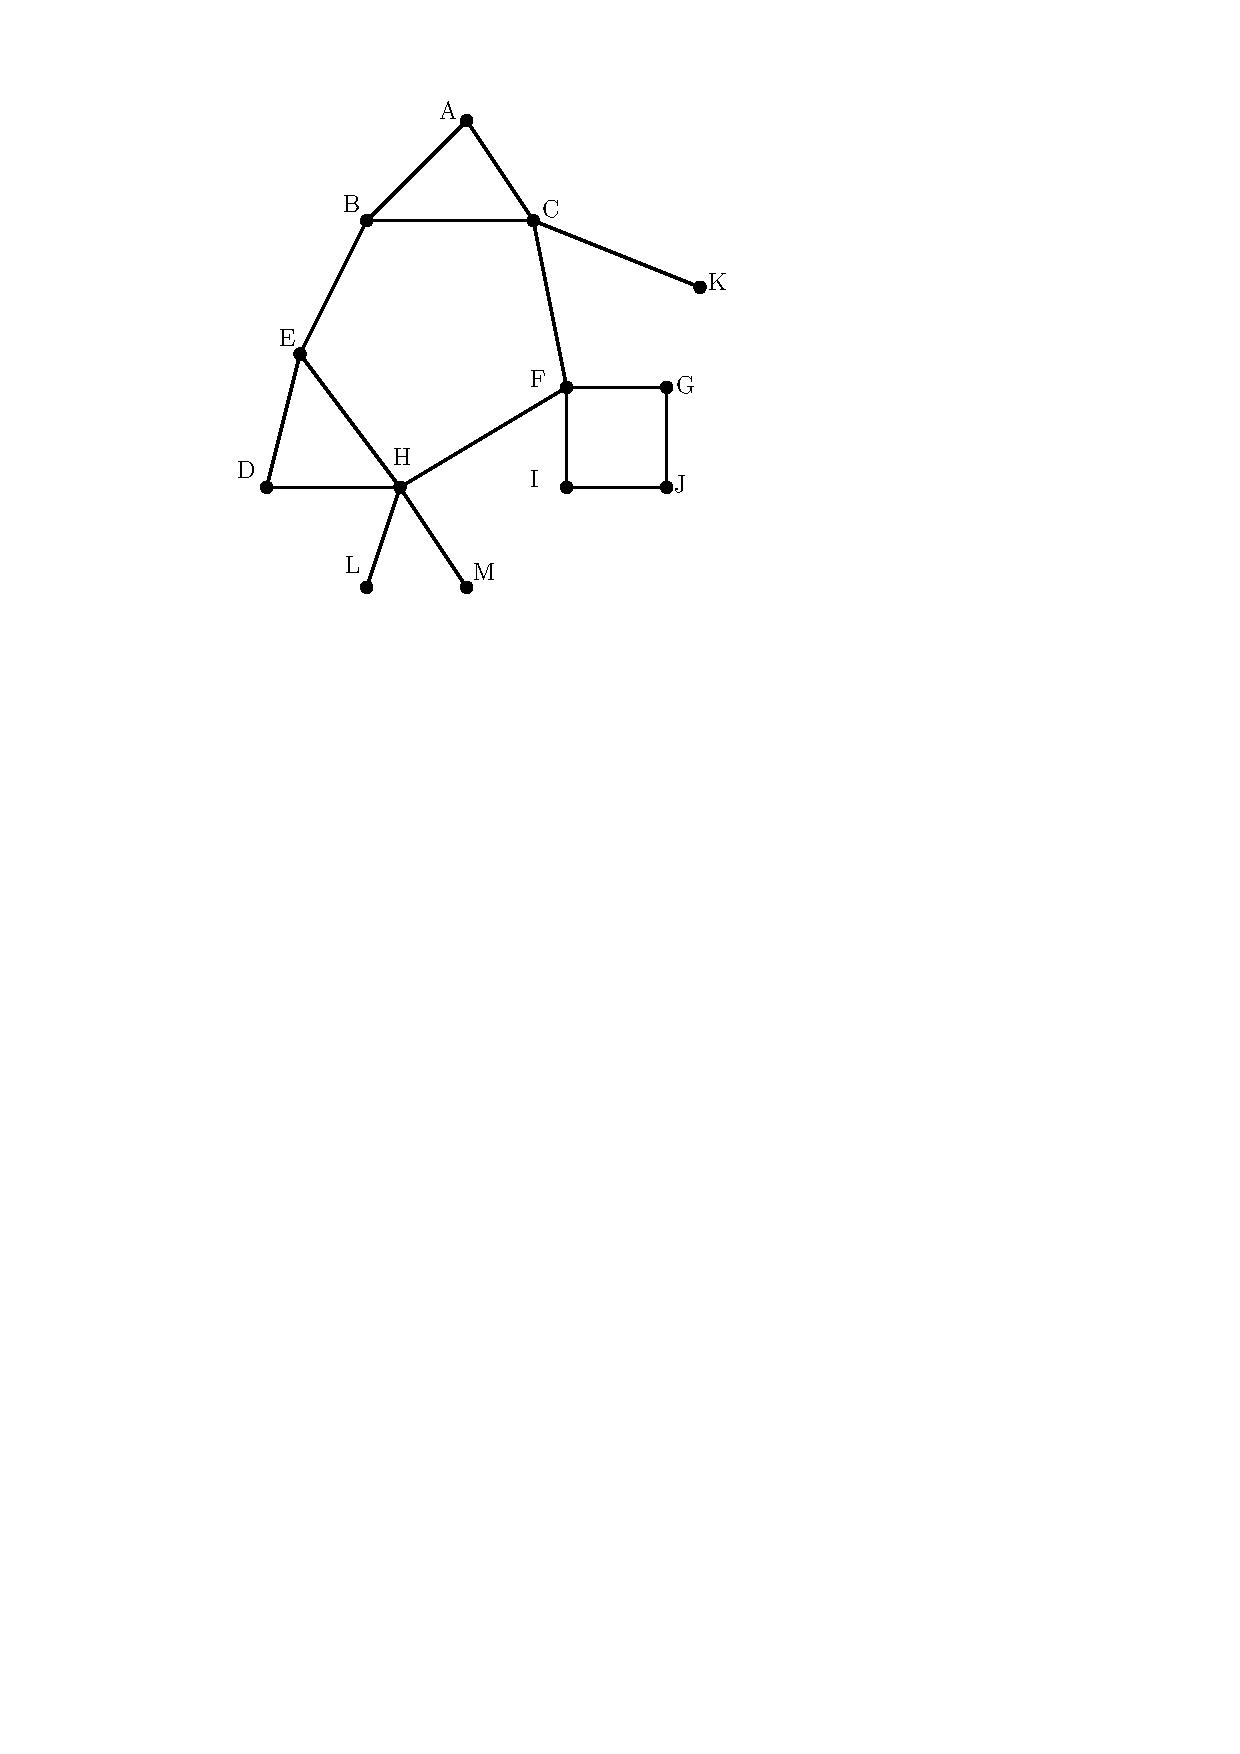
\includegraphics[width=0.4\textwidth]{images/BFS.pdf}
    \caption{An example graph}
    \label{fig:box}
\end{figure}
\begin{solution}
\textit{Claim. }Let $G$ be an undirected graph. Then there exists $k\in\mathbb{Z}$ such that \[\sum_{v\in V}{d_G(v)}=2k,\] where $d(v)$ denotes the degree of vertex $v\in V$ in graph $G$.\\

\noindent\textit{Proof. }We can demonstrate the claim by structural induction on $G$.\\

\noindent\textit{Basis. }Consider $G=(V,\emptyset)$. Then there are no edges in $G$, so for all $v\in V$, we have $d_G(v)=0$. Thus \[\sum_{v\in V}{d_G(v)}=\sum_{v\in V}0=0=2\cdot 0,\]
so the claim holds in the base case.\\

\noindent\textit{Hypothesis. }Consider $G=H=(V,E)$ where $E\neq\emptyset$. Assume that the sum of the degrees of all vertices in graph $H$ is even.\\

\noindent\textit{Inductive step. }Consider $G=(V,E\cup\{\{u,v\}\})$ where $u,v\in V$ and $\{u,v\}\notin E$. Observe
\begin{align*}
\sum_{w\in V}{d_H(w)}
&=d_H(u)+d_H(v)+\sum_{w\in V\setminus\{u,v\}}(d_H(w))\\
&=d_H(u)+d_H(v)+\sum_{w\in V\setminus\{u,v\}}(d_G(w))&\textit{since no $w\in V\setminus\{u,v\}$ is in the new edge,}\\
&=(d_G(u)+1)+(d_G(v)+1)+\sum_{w\in V\setminus\{u,v\}}(d_G(w))&\textit{since $u,v\in\{u,v\}$ but $\{u,v\}\notin E$,}\\
&=2+d_G(u)+d_G(v)+\sum_{w\in V\setminus\{u,v\}}(d_G(w))\\
&=2+\sum_{w\in V}(d_G(w))\\
&=2+2k&\textit{by the inductive hypothesis}\\
&=2(k+1)&\textit{thus completing the inductive step.}
\end{align*}
\noindent Hence, by structural induction, the sum of the degrees of all vertices in an undirected graph is even.$~\square$
\end{solution}
\newpage
\subsection{Depth-first search}

\begin{enumerate}
\item 
Consider the graph in Figure~\ref{fig:box2}. Say we begin a DFS traversal starting at node $A$. List the discovery time (i.e., when we mark a node ``gray'') and finishing time (i.e., when we mark a node ``black'') of each vertex (you may assume each successive step in the traversal takes time 1). Assume that the adjacency lists in the representation of the input graph are in alphabetical order.
\begin{figure}[h!]
\centering
    \begin{tikzpicture}[node distance={20mm}, thick,main/.style={circle, thick,draw,font=\sffamily\bfseries}, ar/.style={-{Stealth[scale=1.2]}}]
          \node[main] (1) {$A$}; 
          \node[main] (2) [below left of=1]{$B$};
          \node[main] (3) [below right of=1]{$C$};
          \node[main] (4) [below of=1]{$D$};
          \node[main] (5) [below left of=4]{$E$};
          \node[main] (6) [below right of=4]{$F$};
          \node[main] (7) [below of=4]{$G$};
          \node[main] (8) [below left of=7]{$H$};
          \node[main] (9) [below right of=7]{$I$};
          
          \draw[ar] (1) -- (2);
          \draw[ar] (3) -- (1);
          \draw[ar] (4) -- (3);
          \draw[ar] (2) -- (5);
          \draw[ar] (7) -- (4);
          \draw[ar] (5) -- (7);
          \draw[ar] (5) -- (8);
          \draw[ar] (9) -- (8);
          \draw[ar] (6) -- (9);
          \draw[ar] (3) -- (6);
          \draw[ar] (4) -- (2);
          \draw[ar] (7) -- (6);
          
    \end{tikzpicture}
    \caption{Graph for Question 2.1}
          \label{fig:box2}
\centering
\end{figure}
    \begin{center}
    \begin{tabular}{|c|c|c|c|c|c|c|c|c|c|}
    \hline
         Node & A & B & C & D & E & F & G & H & I\\
         \hline 
         $d$-time & 1 & 2 & 6 & 5 & 3 & 7 & 4 & 9 & 8 \\
         \hline
         $f$-time & 18 & 17 & 13 & 14 & 16 & 12 & 15 & 10 & 11 \\
         \hline
    \end{tabular}
    \end{center}
\begin{solution}
We can step through the depth-first search algorithm, collecting the times of discovery and finishing for each vertex visited. Visiting adjacent vertices in alphabetical order, we obtain the table above.
\end{solution}
\end{enumerate}    
\newpage
\noindent
As in the previous question, for any vertex $a$ in a directed graph $G$, we denote by $a.\mathsf{d} $ the time at which DFS on $G$ discovers (i.e., marks as ``gray'') the vertex $a$. Similarly, denote by $a.\mathsf{f} $ the time at which DFS fully explores (i.e., marks as ``black'') the vertex $a$. Give counterexamples to the following statements:
\begin{enumerate}[start=2]
    \item If a directed graph $G$ contains a path
    from $a$ to $b$, and if $a.\mathsf{d} < b.\mathsf{d}$ in a depth-first search of $G$, then $b$ is a descendant
    of $a$ in the depth-first forest produced.

\begin{solution}
\textit{False claim. }Let $G=(V,E)$ be a directed graph such that for $a,b\in V$, there exist a path $(a,\dots,b)$. If $a.\mathsf{d}<b.\mathsf{d}$ in a depth-first search of $G$, then $b$ is a descendant of $a$ in the depth-first forest produced. We assume, without loss of generality, that adjacency lists are sorted in alphabetical order.

\textit{Counterexample. }Suppose $G=(\{{\rm X},{\rm Y},{\rm Z}\},\{({\rm X},{\rm Y}),({\rm X},{\rm Z}),({\rm Y},{\rm X})\})$.

Note there exists a path $({\rm Y},{\rm X},{\rm Z})$ from vertex Y to vertex Z. First, we visit X, so ${\rm X}.\mathsf{d}=1$. Then, based on our assumption, we visit ${\rm Y}$, so ${\rm Y}.\mathsf{d}=2$. Upon completing ${\rm Y}$, we have ${\rm Y}.\mathsf{f}=3$. Then, we visit ${\rm Z}$, so ${\rm Z}.\mathsf{d}=4$. Upon completing ${\rm Z}$, we have ${\rm Z}.\mathsf{f}=5$. Finally, we complete ${\rm X}$, giving ${\rm X}.\mathsf{f}=6$. Thus, ${\rm Y}.\mathsf{d}<{\rm Z}.\mathsf{d}$.

However, Y is not a descendant of Z. Hence disproven.$~\square$
\end{solution}
\item If a directed graph $G$ contains a path from $a$ to $b$, then any depth-first search must result in $b.\mathsf{d} < a.\mathsf{f}$.
\begin{solution}
\textit{False claim. }Let $G=(V,E)$ be a directed graph such that for $a,b\in V$, there exist a path $(a,\dots,b)$. Then $b.\mathsf{d}<a.\mathsf{f}$ in a depth-first search of $G$. We assume, without loss of generality, that adjacency lists are sorted in alphabetical order.

\textit{Counterexample. }Suppose $G=(\{{\rm X},{\rm Y},{\rm Z}\},\{({\rm X},{\rm Y}),({\rm X},{\rm Z}),({\rm Y},{\rm X})\})$.

There exists a path $({\rm Y},{\rm X},{\rm Z})$ from vertex Y to vertex Z.

First, we visit X, so ${\rm X}.\mathsf{d}=1$. Then, based on our assumption, we visit ${\rm Y}$, so ${\rm Y}.\mathsf{d}=2$. Upon completing ${\rm Y}$, we have ${\rm Y}.\mathsf{f}=3$. Then, we visit ${\rm Z}$, so ${\rm Z}.\mathsf{d}=4$. Upon completing ${\rm Z}$, we have ${\rm Z}.\mathsf{f}=5$. Finally, we complete ${\rm X}$, giving ${\rm X}.\mathsf{f}=6$. 

Of course, ${\rm Z}.\mathsf{d}\nless{\rm Y}.\mathsf{d}$. Hence disproven.$~\square$
\end{solution}
\end{enumerate}
\newpage
\subsection{2-Colorings}
A \emph{2-coloring} of an undirected graph $G = (V,E)$ assigns each node $v \in V$ a color $v.color \in \{red,green\}$ such that $u.color \neq v.color$ for all $\{u,v\}\in E$. We say the graph $G$ is 2-colorable if such a 2-coloring exists.

\begin{enumerate}
    \item 
    Show that if $G$ is a tree (i.e., connected and acyclic), then there always exists a 2-coloring. How many different 2-colors exist for such a graph?

\begin{solution}
\textit{Claim. }Let $G$ be an undirected graph. If $G$ is a tree, then there exists a 2-coloring of $G$.

\textit{Proof. }Suppose $G$ is a tree. We can demonstrate the claim by structural induction on $G$.

\textit{Basis. }Consider $G=(\emptyset,E)$. Of course, since there are no vertices, $E=\emptyset$. There are no vertices and no edges, so the claim holds vacuously.

Consider $G=(\{v_0\},E)$. Since $G$ is a tree, $G$ is acyclic, and thus $E=\emptyset$. We may color $v_0$ red or green to produce a 2-coloring of graph $G$.

The claim holds in the base cases.

\textit{Hypothesis. }Consider $G=(V,E)$ where $|V|>1$. Assume that there exists a 2-coloring of graph $H$.

\textit{Inductive step. }Consider $G=(V\cup\{v\},E)$ where $v\notin V$. Since $G$ is a tree, $G$ is connected. Since $|V|>1$, there exists $u\in V$ where $\{u,v\}\in E$. Since $G$ is a tree, there is only one such $u$.

From the inductive hypothesis, there exists a 2-coloring of $H$. In this coloring, either $u$ 
\end{solution}


	\item 
	Describe how to modify the algorithm for Depth First Search so that it assigns a valid 2-coloring, or returns an error in case none exists. To this end, write a function {\sc TwoColoring-Visit}$(G,u,c)$ that takes a graph $G$, a vertex $u$, and a color $c \in \{red,green\}$ such that the following driver function either assigns a valid 2-coloring and returns $success$, or returns $error$ in case no 2-coloring exists. Your algorithm should assume $G$ to be represented as an adjacency list and run in $O(|V| + |E|)$. 
	
	\begin{code}
		{\sc TwoColoring}$(G)$\\
		\> \For $u \in G.V$ \Do \\
		\> \> $u.color = white$ \\
		\> \For $u \in G.V$ \Do \\
		\> \> \If $u.color \stackrel{?}{=} white$ \Then \\
		\> \> \> $\text{\sc TwoColoring-Visit}(G,u,red)$ \\
		\> \Return $success$ \\
	\end{code}

\begin{solution}   INSERT YOUR SOLUTION HERE   \end{solution}

    \item Prove the correctness of your algorithm. More concretely, show (a) that the assigned coloring is always a valid 2-coloring, and (b) if a 2-coloring exists then the algorithm does assign one.
    \hint{Consider the DFS tree and the edge classification. You may reuse ideas from the first subproblem.}
    
\begin{solution}   INSERT YOUR SOLUTION HERE   \end{solution}
\end{enumerate}
